\section{Discussion and Future Work}
\label{sec:discuss} In this section, we discuss related issues of
our approach.

\textbf{Aligning client code of similar functionalities.} As shown
in Table~\ref{table:analyzingclient}, our approach sometimes fails
to align client code. For some considerations, programmers may
implement one functionality as one class or one method in one
language version but implement the same functionality as multiple
classes or methods in another language version. One feasible way to
align these functionalities is to analyze them dynamically. For
example, Jiang and Su~\cite{jiang2009automatic} propose an approach
to mine code snippets of similar functionalities. We plan to develop
a dynamic technique for those unmatched classes or methods in our
future work.
\begin{figure}[t]
\centering
\includegraphics[scale=1,clip]{figure/n2n.eps}\vspace*{-3ex}
 \caption{Merging technique}\vspace*{-3.5ex}
 \label{fig:n2n}
\end{figure}

\textbf{Mining richer API mapping.} As shown in
Table~\ref{table:compare}, although we use 10 large projects as
subjects, our evaluation does not achieve high recalls for J2SE. For
a given library, these projects still do not provide adequate source
files for mining. Our previous
work~\cite{thummalapenta07parseweb,thummalapentaase08spotweb} shows
that it is feasible to use the internet-scale open source code
available on the web as subjects for mining with the help of code
search engines such as Google code
search\footnote{\url{http://www.google.com/codesearch}}. We plan to
leverage those search engines to mine richer API mapping in our
future work.

\textbf{Ranking mined mapping relations.} When comparing with the
built mapping files of CSharp2Java, we choose mined mapping
relations of APIs with the highest supports as generated mapping
files. However, in some cases, the API mapping with the highest
support is not necessarily the best choice. For example,
\CodeIn{java.util. ArrayList} is mapped to
\CodeIn{System.Collections.ArrayList} based on support values. The
Java class supports generic programming, whereas the C\# class does
not. Consequently, the Java class seems to be better mapped to
\CodeIn{System.Collections.Generic.List} as this C\# class also
supports generic programming. We plan to develop ranking techniques
to address this issue in future work.

\textbf{Mining more many-to-many mapping relations of API methods.}
A majority of mined mapping relations of API methods describe
one-to-one relations. Algorithm 2 merges the next API method with a
forward strategy. For the example shown in Figure~\ref{fig:n2n}, if
the algorithm merges \CodeIn{method1()} and \CodeIn{method2()} but
fails to find a match, the algorithm tries to merge
\CodeIn{method3()}. In some cases, a match can be found if the
algorithm merges \CodeIn{method4()} instead of \CodeIn{method3()}.
We plan to improve the algorithm to mine more many-to-many relations
in future work.

\textbf{Migrating many-to-many mapping relations of API methods.} A
mined many-to-many mapping of API methods may have multiple outputs
and complicated internal data processes. Our defined API
transformation graphs help find out all essential API methods.
However a graph does not describe adequate details to support
automatic translation. For example, we need to manually add an
\emph{or} operator for the two outputs of the API mapping shown in
Figure~\ref{fig:example}. We plan to add more details to help
automate migration with many-to-many mapping relations in future
work.

\textbf{Migrating unmapped APIs.} Our approach mines API mapping of
methods that have mapped inputs, mapped outputs, and similar
functionalities. Consequently, mined API mapping can be migrated
automatically. However, some APIs between two languages cannot
satisfy all the three criteria. For these APIs, if outputs are
unmapped, our approach can simply ignore outputs when outputs are
not used in client code. If inputs or functionalities are unmapped,
we plan to develop techniques that analyze how two versions of a
project deal with a similar unmapped API problem for some reusable
code snippets in future work.
